
\documentclass[standalone]{beamer}

\begin{document}
\section{基礎線段樹}

\begin{frame}{\btitle{例題}}
  \begin{problem}[區間最大值 Range Maximum Query,RMQ]
    給定一個長度為 \(N\) 的正整數序列 \(a_1, \dots, a_N\),接著有 \(Q\) 個詢問,每個詢問形如
    \begin{itemize}
        \item
            \(\texttt{1 l r}\),請你回答在 \(a_l, a_{l+1}, \dots, a_{r}\) 當中的最大值。
        \item
            \(\texttt{2 p x}\),請你把 \(a_p\) 修改為 \(x\)。
    \end{itemize}
    
    \begin{itemize}
        \item
            \(N, Q \leq 5 \times 10^5\)
    \end{itemize}
  \end{problem}
\end{frame}

\begin{frame}{\btitle{例題}}
  \begin{itemize}
    \item 從前面的經驗來看,我們好像要對序列做一些事情,才能解決這題
    \item 前面介紹的 Sparse Table 已經派不上用場了
    \begin{itemize}
      \item 因為修改一個元素會動到將近 $O(N)$ 個預處理表格的內容 
    \end{itemize}
    \item 但 Sparse Table 的精神可以給我們一些啟發:
    \begin{itemize}
      \item 答案是從某些預處理資料組合出來的
      \item 預處理資料盡量可以由本身小資料算出大資料的答案
      \item 大資料底下的小資料大小大概都是大資料的一半
    \end{itemize}
    \item 除了 Sparse Table 精神外,我們還要支援:
    \begin{itemize}
      \item 修改一個元素的時候,讓包含這個元素的資料盡量少
    \end{itemize}
  \end{itemize}
\end{frame}

\begin{frame}{\btitle{例題}}
  \begin{itemize}
    \item \textbf{大資料底下的小資料大小大概都是大資料的一半}
    \item 不妨試試看分治吧!來看一個長度為 $5$ 的序列的分治過程
      \begin{figure}
        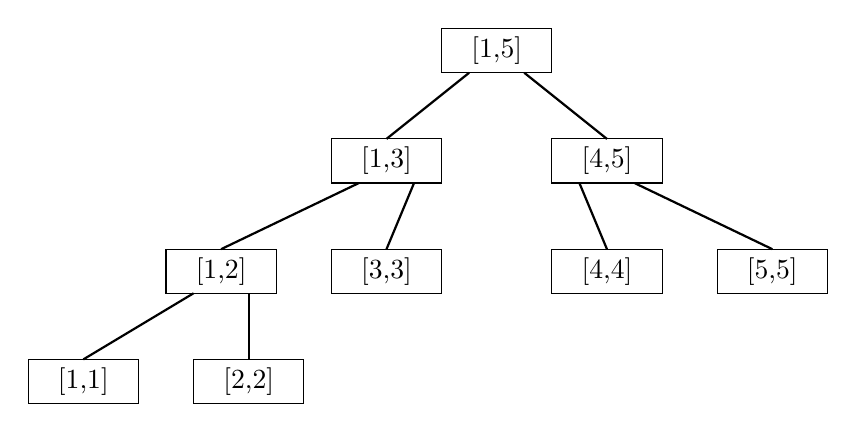
\begin{tikzpicture}[scale=0.7]
          \draw [black] (-1,7.9) rectangle (1,7.1) node [black, midway] {[1,5]}; % Draws a rectangle

          \draw [black] (-3,5.9) rectangle (-1,5.1) node [black,midway] {[1,3]}; % Draws a rectangle
          \draw [black] (1,5.9) rectangle (3,5.1) node [black,midway] {[4,5]}; % Draws a rectangle

          \draw [black] (-6,3.9) rectangle (-4,3.1) node [black,midway] {[1,2]}; % Draws a rectangle
          \draw [black] (-3,3.9) rectangle (-1,3.1) node [black,midway] {[3,3]}; % Draws a rectangle
          \draw [black] (1,3.9) rectangle (3,3.1) node [black,midway] {[4,4]}; % Draws a rectangle
          \draw [black] (4,3.9) rectangle (6,3.1) node [black,midway] {[5,5]}; % Draws a rectangle

          \draw [black] (-8.5,1.9) rectangle (-6.5,1.1) node [black,midway] {[1,1]}; % Draws a rectangle
          \draw [black] (-5.5,1.9) rectangle (-3.5,1.1) node [black,midway] {[2,2]}; % Draws a rectangle

          \draw [thick] (-0.5,7.1) to (-2,5.9);
          \draw [thick] (0.5,7.1) to (2,5.9);

          \draw [thick] (-2.5,5.1) to (-5,3.9);
          \draw [thick] (-1.5,5.1) to (-2,3.9);

          \draw [thick] (1.5,5.1) to (2,3.9);
          \draw [thick] (2.5,5.1) to (5,3.9);

          \draw [thick] (-5.5,3.1) to (-7.5,1.9);
          \draw [thick] (-4.5,3.1) to (-4.5,1.9);
          % \draw [thick] (-2,2) % Draws a line
          % to [out=10,in=190] (2,2)
          % to [out=10,in=90] (6,0) 
          % to [out=-90,in=30] (-2,-2);    
        \end{tikzpicture}
      \end{figure}
  \end{itemize}
\end{frame}

\begin{frame}{基礎線段樹}
  \begin{itemize}
    \item 把這個結構存成樹,並假設每個節點都存該區間的最大值。以下假設 $a = [1, 16, 2, 8, 4]$
      \begin{figure}
        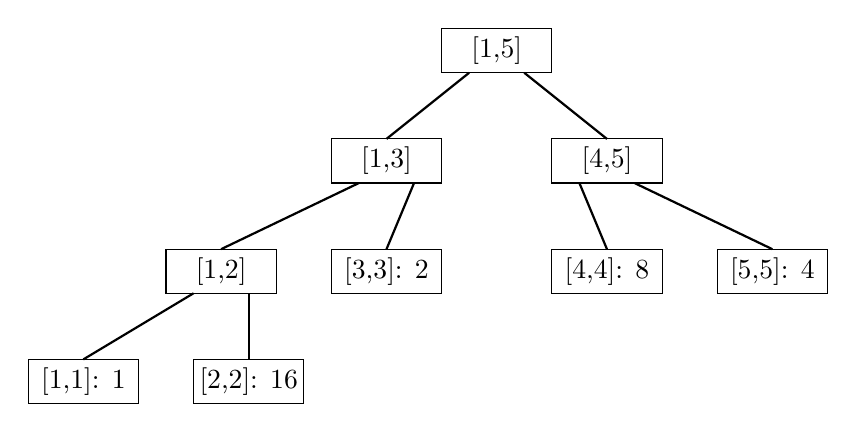
\begin{tikzpicture}[scale=0.7]
          \draw [black] (-1,7.9) rectangle (1,7.1) node [black, midway] {[1,5]}; % Draws a rectangle

          \draw [black] (-3,5.9) rectangle (-1,5.1) node [black,midway] {[1,3]}; % Draws a rectangle
          \draw [black] (1,5.9) rectangle (3,5.1) node [black,midway] {[4,5]}; % Draws a rectangle

          \draw [black] (-6,3.9) rectangle (-4,3.1) node [black,midway] {[1,2]}; % Draws a rectangle
          \draw [black] (-3,3.9) rectangle (-1,3.1) node [black,midway] {[3,3]: 2}; % Draws a rectangle
          \draw [black] (1,3.9) rectangle (3,3.1) node [black,midway] {[4,4]: 8}; % Draws a rectangle
          \draw [black] (4,3.9) rectangle (6,3.1) node [black,midway] {[5,5]: 4}; % Draws a rectangle

          \draw [black] (-8.5,1.9) rectangle (-6.5,1.1) node [black,midway] {[1,1]: 1}; % Draws a rectangle
          \draw [black] (-5.5,1.9) rectangle (-3.5,1.1) node [black,midway] {[2,2]: 16}; % Draws a rectangle

          \draw [thick] (-0.5,7.1) to (-2,5.9);
          \draw [thick] (0.5,7.1) to (2,5.9);

          \draw [thick] (-2.5,5.1) to (-5,3.9);
          \draw [thick] (-1.5,5.1) to (-2,3.9);

          \draw [thick] (1.5,5.1) to (2,3.9);
          \draw [thick] (2.5,5.1) to (5,3.9);

          \draw [thick] (-5.5,3.1) to (-7.5,1.9);
          \draw [thick] (-4.5,3.1) to (-4.5,1.9);
          % \draw [thick] (-2,2) % Draws a line
          % to [out=10,in=190] (2,2)
          % to [out=10,in=90] (6,0) 
          % to [out=-90,in=30] (-2,-2);    
        \end{tikzpicture}
      \end{figure}
  \end{itemize}
\end{frame}

\begin{frame}{基礎線段樹}
  \begin{itemize}
    \item 把這個結構存成樹,並假設每個節點都存該區間的最大值。以下假設 $a = [1, 16, 2, 8, 4]$
      \begin{figure}
        \begin{tikzpicture}[scale=0.7]
          \draw [black] (-1,7.9) rectangle (1,7.1) node [black, midway] {[1,5]}; % Draws a rectangle

          \draw [black] (-3,5.9) rectangle (-1,5.1) node [black,midway] {[1,3]}; % Draws a rectangle
          \draw [red] (1,5.9) rectangle (3,5.1) node [red,midway] {[4,5]: 8}; % Draws a rectangle

          \draw [red] (-6,3.9) rectangle (-4,3.1) node [red,midway] {[1,2]: 16}; % Draws a rectangle
          \draw [black] (-3,3.9) rectangle (-1,3.1) node [black,midway] {[3,3]: 2}; % Draws a rectangle
          \draw [black] (1,3.9) rectangle (3,3.1) node [black,midway] {[4,4]: 8}; % Draws a rectangle
          \draw [black] (4,3.9) rectangle (6,3.1) node [black,midway] {[5,5]: 4}; % Draws a rectangle

          \draw [black] (-8.5,1.9) rectangle (-6.5,1.1) node [black,midway] {[1,1]: 1}; % Draws a rectangle
          \draw [black] (-5.5,1.9) rectangle (-3.5,1.1) node [black,midway] {[2,2]: 16}; % Draws a rectangle

          \draw [thick] (-0.5,7.1) to (-2,5.9);
          \draw [thick] (0.5,7.1) to (2,5.9);

          \draw [thick] (-2.5,5.1) to (-5,3.9);
          \draw [thick] (-1.5,5.1) to (-2,3.9);

          \draw [red, arrows={Latex[length=3mm]}-] (1.5,5.1) -- (2,3.9);
          \draw [red, arrows={Latex[length=3mm]}-] (2.5,5.1) -- (5,3.9);

          \draw [red, arrows={Latex[length=3mm]}-] (-5.5,3.1) -- (-7.5,1.9);
          \draw [red, arrows={Latex[length=3mm]}-] (-4.5,3.1) -- (-4.5,1.9);
          % \draw [thick] (-2,2) % Draws a line
          % to [out=10,in=190] (2,2)
          % to [out=10,in=90] (6,0) 
          % to [out=-90,in=30] (-2,-2);    
        \end{tikzpicture}
      \end{figure}
  \end{itemize}
\end{frame}

\begin{frame}{基礎線段樹}
  \begin{itemize}
    \item 把這個結構存成樹,並假設每個節點都存該區間的最大值。以下假設 $a = [1, 16, 2, 8, 4]$
      \begin{figure}
        \begin{tikzpicture}[scale=0.7]
          \draw [black] (-1,7.9) rectangle (1,7.1) node [black, midway] {[1,5]}; % Draws a rectangle

          \draw [red] (-3,5.9) rectangle (-1,5.1) node [red,midway] {[1,3]: 16}; % Draws a rectangle
          \draw [black] (1,5.9) rectangle (3,5.1) node [black,midway] {[4,5]: 8}; % Draws a rectangle

          \draw [black] (-6,3.9) rectangle (-4,3.1) node [black,midway] {[1,2]: 16}; % Draws a rectangle
          \draw [black] (-3,3.9) rectangle (-1,3.1) node [black,midway] {[3,3]: 2}; % Draws a rectangle
          \draw [black] (1,3.9) rectangle (3,3.1) node [black,midway] {[4,4]: 8}; % Draws a rectangle
          \draw [black] (4,3.9) rectangle (6,3.1) node [black,midway] {[5,5]: 4}; % Draws a rectangle

          \draw [black] (-8.5,1.9) rectangle (-6.5,1.1) node [black,midway] {[1,1]: 1}; % Draws a rectangle
          \draw [black] (-5.5,1.9) rectangle (-3.5,1.1) node [black,midway] {[2,2]: 16}; % Draws a rectangle

          \draw [thick] (-0.5,7.1) to (-2,5.9);
          \draw [thick] (0.5,7.1) to (2,5.9);

          \draw [red, arrows={Latex[length=3mm]}-] (-2.5,5.1) -- (-5,3.9);
          \draw [red, arrows={Latex[length=3mm]}-] (-1.5,5.1) -- (-2,3.9);

          \draw [thick] (1.5,5.1) to (2,3.9);
          \draw [thick] (2.5,5.1) to (5,3.9);

          \draw [thick] (-5.5,3.1) to (-7.5,1.9);
          \draw [thick] (-4.5,3.1) to (-4.5,1.9);
          % \draw [thick] (-2,2) % Draws a line
          % to [out=10,in=190] (2,2)
          % to [out=10,in=90] (6,0) 
          % to [out=-90,in=30] (-2,-2);    
        \end{tikzpicture}
      \end{figure}
  \end{itemize}
\end{frame}

\begin{frame}{基礎線段樹}
  \begin{itemize}
    \item 把這個結構存成樹,並假設每個節點都存該區間的最大值。以下假設 $a = [1, 16, 2, 8, 4]$
      \begin{figure}
        \begin{tikzpicture}[scale=0.7]
          \draw [red] (-1,7.9) rectangle (1,7.1) node [red, midway] {[1,5]: 16}; % Draws a rectangle

          \draw [black] (-3,5.9) rectangle (-1,5.1) node [black,midway] {[1,3]: 16}; % Draws a rectangle
          \draw [black] (1,5.9) rectangle (3,5.1) node [black,midway] {[4,5]: 8}; % Draws a rectangle

          \draw [black] (-6,3.9) rectangle (-4,3.1) node [black,midway] {[1,2]: 16}; % Draws a rectangle
          \draw [black] (-3,3.9) rectangle (-1,3.1) node [black,midway] {[3,3]: 2}; % Draws a rectangle
          \draw [black] (1,3.9) rectangle (3,3.1) node [black,midway] {[4,4]: 8}; % Draws a rectangle
          \draw [black] (4,3.9) rectangle (6,3.1) node [black,midway] {[5,5]: 4}; % Draws a rectangle

          \draw [black] (-8.5,1.9) rectangle (-6.5,1.1) node [black,midway] {[1,1]: 1}; % Draws a rectangle
          \draw [black] (-5.5,1.9) rectangle (-3.5,1.1) node [black,midway] {[2,2]: 16}; % Draws a rectangle

          \draw [red, arrows={Latex[length=3mm]}-] (-0.5,7.1) -- (-2,5.9);
          \draw [red, arrows={Latex[length=3mm]}-] (0.5,7.1) -- (2,5.9);

          \draw [thick] (-2.5,5.1) to (-5,3.9);
          \draw [thick] (-1.5,5.1) to (-2,3.9);

          \draw [thick] (1.5,5.1) to (2,3.9);
          \draw [thick] (2.5,5.1) to (5,3.9);

          \draw [thick] (-5.5,3.1) to (-7.5,1.9);
          \draw [thick] (-4.5,3.1) to (-4.5,1.9);
          % \draw [thick] (-2,2) % Draws a line
          % to [out=10,in=190] (2,2)
          % to [out=10,in=90] (6,0) 
          % to [out=-90,in=30] (-2,-2);    
        \end{tikzpicture}
      \end{figure}
  \end{itemize}
\end{frame}

\begin{frame}{基礎線段樹}
  \begin{itemize}
    \item $a = [1, 16, 2, 8, 4]$
      \begin{figure}
        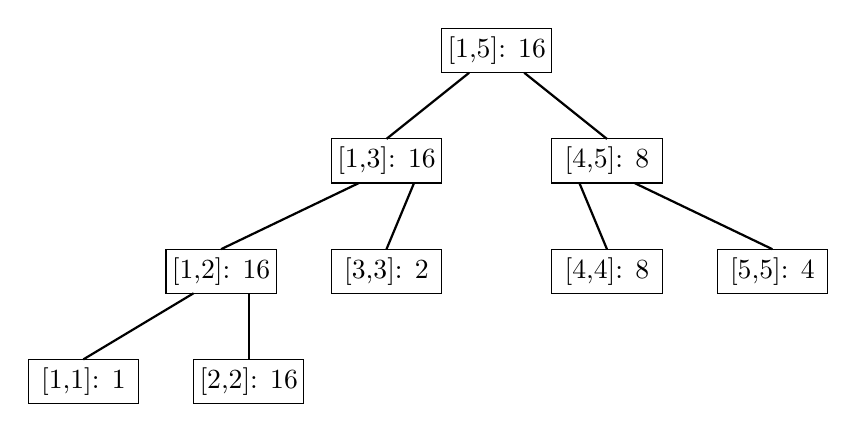
\begin{tikzpicture}[scale=0.7]
          \draw [black] (-1,7.9) rectangle (1,7.1) node [black, midway] {[1,5]: 16}; % Draws a rectangle

          \draw [black] (-3,5.9) rectangle (-1,5.1) node [black,midway] {[1,3]: 16}; % Draws a rectangle
          \draw [black] (1,5.9) rectangle (3,5.1) node [black,midway] {[4,5]: 8}; % Draws a rectangle

          \draw [black] (-6,3.9) rectangle (-4,3.1) node [black,midway] {[1,2]: 16}; % Draws a rectangle
          \draw [black] (-3,3.9) rectangle (-1,3.1) node [black,midway] {[3,3]: 2}; % Draws a rectangle
          \draw [black] (1,3.9) rectangle (3,3.1) node [black,midway] {[4,4]: 8}; % Draws a rectangle
          \draw [black] (4,3.9) rectangle (6,3.1) node [black,midway] {[5,5]: 4}; % Draws a rectangle

          \draw [black] (-8.5,1.9) rectangle (-6.5,1.1) node [black,midway] {[1,1]: 1}; % Draws a rectangle
          \draw [black] (-5.5,1.9) rectangle (-3.5,1.1) node [black,midway] {[2,2]: 16}; % Draws a rectangle

          \draw [thick] (-0.5,7.1) to (-2,5.9);
          \draw [thick] (0.5,7.1) to (2,5.9);

          \draw [thick] (-2.5,5.1) to (-5,3.9);
          \draw [thick] (-1.5,5.1) to (-2,3.9);

          \draw [thick] (1.5,5.1) to (2,3.9);
          \draw [thick] (2.5,5.1) to (5,3.9);

          \draw [thick] (-5.5,3.1) to (-7.5,1.9);
          \draw [thick] (-4.5,3.1) to (-4.5,1.9);
          % \draw [thick] (-2,2) % Draws a line
          % to [out=10,in=190] (2,2)
          % to [out=10,in=90] (6,0) 
          % to [out=-90,in=30] (-2,-2);    
        \end{tikzpicture}
      \end{figure}
    \item 答案是從某些預處理資料組合出來的:不知道可不可行
    \item 大資料都可以由小資料構成、小資料大小大概是大資料兩倍:可以
  \end{itemize}
\end{frame}

\begin{frame}{基礎線段樹}
  \begin{itemize}
    \item $a = [1, 16, 2, 8, 4]$
      \begin{figure}
        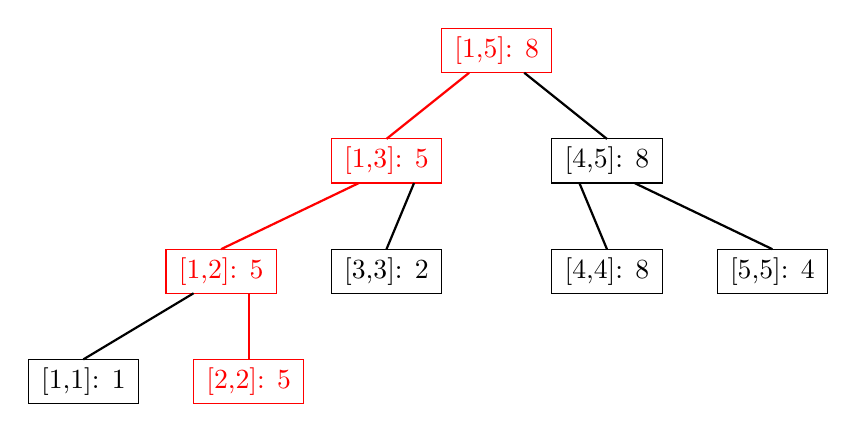
\begin{tikzpicture}[scale=0.7]
          \draw [red] (-1,7.9) rectangle (1,7.1) node [red, midway] {[1,5]: 8}; % Draws a rectangle

          \draw [red] (-3,5.9) rectangle (-1,5.1) node [red,midway] {[1,3]: 5}; % Draws a rectangle
          \draw [black] (1,5.9) rectangle (3,5.1) node [black,midway] {[4,5]: 8}; % Draws a rectangle

          \draw [red] (-6,3.9) rectangle (-4,3.1) node [red,midway] {[1,2]: 5}; % Draws a rectangle
          \draw [black] (-3,3.9) rectangle (-1,3.1) node [black,midway] {[3,3]: 2}; % Draws a rectangle
          \draw [black] (1,3.9) rectangle (3,3.1) node [black,midway] {[4,4]: 8}; % Draws a rectangle
          \draw [black] (4,3.9) rectangle (6,3.1) node [black,midway] {[5,5]: 4}; % Draws a rectangle

          \draw [black] (-8.5,1.9) rectangle (-6.5,1.1) node [black,midway] {[1,1]: 1}; % Draws a rectangle
          \draw [red] (-5.5,1.9) rectangle (-3.5,1.1) node [red,midway] {[2,2]: 5}; % Draws a rectangle

          \draw [thick, red] (-0.5,7.1) to (-2,5.9);
          \draw [thick] (0.5,7.1) to (2,5.9);

          \draw [thick, red] (-2.5,5.1) to (-5,3.9);
          \draw [thick] (-1.5,5.1) to (-2,3.9);

          \draw [thick] (1.5,5.1) to (2,3.9);
          \draw [thick] (2.5,5.1) to (5,3.9);

          \draw [thick] (-5.5,3.1) to (-7.5,1.9);
          \draw [thick, red] (-4.5,3.1) to (-4.5,1.9);
          % \draw [thick] (-2,2) % Draws a line
          % to [out=10,in=190] (2,2)
          % to [out=10,in=90] (6,0) 
          % to [out=-90,in=30] (-2,-2);    
        \end{tikzpicture}
      \end{figure}
    \item 修改一個元素的時候,讓包含這個元素的資料盡量少:好像可以(上圖是修改 $a_2$ 改成 $5$ 的狀況)
  \end{itemize}
\end{frame}

\begin{frame}{基礎線段樹}
  \begin{itemize}
    \item 在繼續下去之前,我們先來看看這棵樹的性質:
      \begin{itemize}
        \item 樹的節點總共有 $2N - 1$ 個
        \item 樹的高度為 $O(\log N)$
        \item 他是二元樹
      \end{itemize}
    \item 把樹上的數值填好只需要花 $O(N)$ 的時間(從葉子一路往上填,父節點的答案從左右子樹更新)
    \item 這種樹我們稱為「線段樹」
    \item 來看看怎麼把樹建出來吧!
  \end{itemize}
\end{frame}

\begin{frame}[fragile]{\btitle{範例實作}}
  \begin{minted}[breaklines]{cpp}
    const int inf = numeric_limits<int>::max();
    struct Node {
      Node *lc, *rc;
      int mx;
      void pull() { mx = max(lc->mx, rc->mx); }
    } *root = nullptr;
  \end{minted}

  \texttt{pull()} 這個函數用途是父節點利用左右子樹的答案更新自己的答案,\textbf{每當任何子樹的值有更動時,都需要重新呼叫這個 function 更新父節點的答案}
\end{frame}

\begin{frame}[fragile]{\btitle{範例實作}}
  \begin{minted}[breaklines]{cpp}
    Node *build(int arr[], int l, int r) { // 回傳區間 [l, r] 這段區間構成的線段樹的根節點
      Node *res = new Node();
      if (l == r) { // 葉節點
        res->lc = res->rc = nullptr;
        res->mx = arr[l];
      } else {
        int m = (l + r) / 2;
        res->lc = build(arr, l, m); // 把左半區間建好的樹接在自己的左子樹上
        res->rc = build(arr, m + 1, r); // 把右半區間建好的樹接在自己的左子樹上
        res->pull(); // 更新父節點資訊
      }
      return res;
    }
  \end{minted}
\end{frame}

\begin{frame}[fragile]{\btitle{範例實作}}
  \begin{itemize}
    \item 線段樹的實作會使用到大量的遞迴!
    \item 在遞迴線段樹節點的時候,通常會把該節點代表的區間(上述 code 的 $l, r$)一起遞迴下去
    \item 線段樹的實作有很多種版本,這裡提供的是指標版
  \end{itemize}
\end{frame}

\begin{frame}{基礎線段樹}
  \begin{itemize}
    \item $a = [1, 16, 2, 8, 4]$
      \begin{figure}
        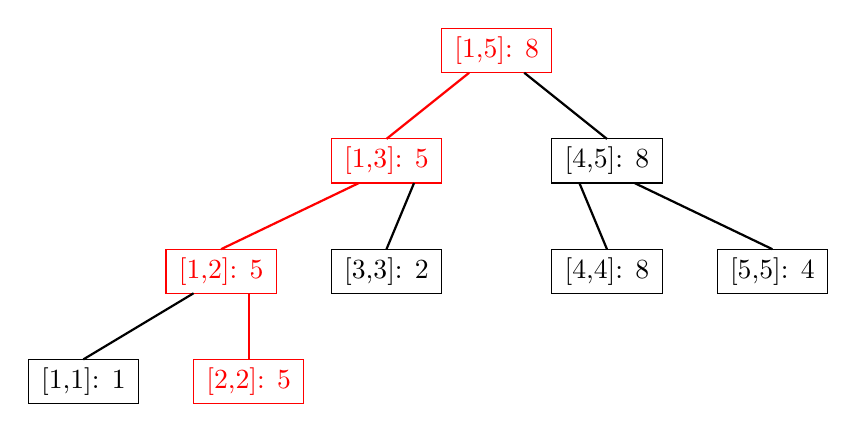
\begin{tikzpicture}[scale=0.7]
          \draw [red] (-1,7.9) rectangle (1,7.1) node [red, midway] {[1,5]: 8}; % Draws a rectangle

          \draw [red] (-3,5.9) rectangle (-1,5.1) node [red,midway] {[1,3]: 5}; % Draws a rectangle
          \draw [black] (1,5.9) rectangle (3,5.1) node [black,midway] {[4,5]: 8}; % Draws a rectangle

          \draw [red] (-6,3.9) rectangle (-4,3.1) node [red,midway] {[1,2]: 5}; % Draws a rectangle
          \draw [black] (-3,3.9) rectangle (-1,3.1) node [black,midway] {[3,3]: 2}; % Draws a rectangle
          \draw [black] (1,3.9) rectangle (3,3.1) node [black,midway] {[4,4]: 8}; % Draws a rectangle
          \draw [black] (4,3.9) rectangle (6,3.1) node [black,midway] {[5,5]: 4}; % Draws a rectangle

          \draw [black] (-8.5,1.9) rectangle (-6.5,1.1) node [black,midway] {[1,1]: 1}; % Draws a rectangle
          \draw [red] (-5.5,1.9) rectangle (-3.5,1.1) node [red,midway] {[2,2]: 5}; % Draws a rectangle

          \draw [thick, red] (-0.5,7.1) to (-2,5.9);
          \draw [thick] (0.5,7.1) to (2,5.9);

          \draw [thick, red] (-2.5,5.1) to (-5,3.9);
          \draw [thick] (-1.5,5.1) to (-2,3.9);

          \draw [thick] (1.5,5.1) to (2,3.9);
          \draw [thick] (2.5,5.1) to (5,3.9);

          \draw [thick] (-5.5,3.1) to (-7.5,1.9);
          \draw [thick, red] (-4.5,3.1) to (-4.5,1.9);
          % \draw [thick] (-2,2) % Draws a line
          % to [out=10,in=190] (2,2)
          % to [out=10,in=90] (6,0) 
          % to [out=-90,in=30] (-2,-2);    
        \end{tikzpicture}
      \end{figure}
    \item 單點修改其實只會從\textbf{葉節點一路修改到根}
    \item 樹高是 $O(\log N)$,所以複雜度為 $O(\log N)$
  \end{itemize}
\end{frame}

\begin{frame}{\btitle{修改二步驟}}
  \begin{itemize}
    \item 修改的位置是 \(p\)
    \item 假設目前的節點儲存的資訊是 \([L, R]\)
    \item 修改二步驟:
    \begin{enumerate}
      \item
        如果 \([L, R]\) 區間長度為 1,可以知道這就是是一個葉節點。
      \item
          否則設 \(M = \lfloor \frac{L+R}{2} \rfloor\),\(p\) 一定在 \([L, M]\) 或是 \([M+1, R]\) 其中之一,依照 \(p\) 與 \(M\) 的關係決定往哪個子樹遞迴。
          在子樹更新完之後,\textbf{更新這個節點的最大值}成為兩個子節點當中較大的。
    \end{enumerate}
  \end{itemize}
\end{frame}

\begin{frame}[fragile]{\btitle{範例實作}}
  \begin{minted}[breaklines]{cpp}
    void modify(Node *nd, int val, int p, int l, int r) {
      if (l == r) { // 葉節點
        nd->mx = val;
        return;
      }
      int m = (l + r) / 2;
      if (p <= m) // 看修改的點是在左邊還是右邊
        modify(nd->lc, val, p, l, m);
      else
        modify(nd->rc, val, p, m + 1, r);
      nd->pull(); // IMPORTANT!!
    }
  \end{minted}
\end{frame}

\begin{frame}[fragile]{\btitle{查詢}}
  \begin{itemize}
    \item 查詢 $[3, 5]$
      \begin{figure}
        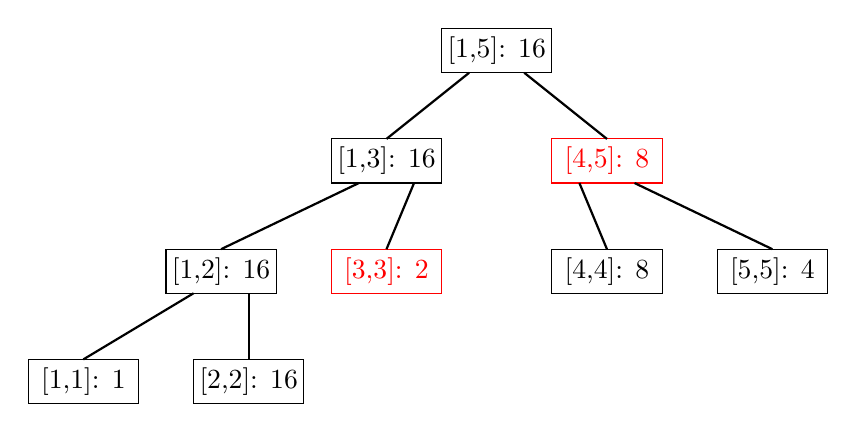
\begin{tikzpicture}[scale=0.7]
          \draw [black] (-1,7.9) rectangle (1,7.1) node [black, midway] {[1,5]: 16}; % Draws a rectangle

          \draw [black] (-3,5.9) rectangle (-1,5.1) node [black,midway] {[1,3]: 16}; % Draws a rectangle
          \draw [red] (1,5.9) rectangle (3,5.1) node [red,midway] {[4,5]: 8}; % Draws a rectangle

          \draw [black] (-6,3.9) rectangle (-4,3.1) node [black,midway] {[1,2]: 16}; % Draws a rectangle
          \draw [red] (-3,3.9) rectangle (-1,3.1) node [red,midway] {[3,3]: 2}; % Draws a rectangle
          \draw [black] (1,3.9) rectangle (3,3.1) node [black,midway] {[4,4]: 8}; % Draws a rectangle
          \draw [black] (4,3.9) rectangle (6,3.1) node [black,midway] {[5,5]: 4}; % Draws a rectangle

          \draw [black] (-8.5,1.9) rectangle (-6.5,1.1) node [black,midway] {[1,1]: 1}; % Draws a rectangle
          \draw [black] (-5.5,1.9) rectangle (-3.5,1.1) node [black,midway] {[2,2]: 16}; % Draws a rectangle

          \draw [thick] (-0.5,7.1) to (-2,5.9);
          \draw [thick] (0.5,7.1) to (2,5.9);

          \draw [thick] (-2.5,5.1) to (-5,3.9);
          \draw [thick] (-1.5,5.1) to (-2,3.9);

          \draw [thick] (1.5,5.1) to (2,3.9);
          \draw [thick] (2.5,5.1) to (5,3.9);

          \draw [thick] (-5.5,3.1) to (-7.5,1.9);
          \draw [thick] (-4.5,3.1) to (-4.5,1.9);
          % \draw [thick] (-2,2) % Draws a line
          % to [out=10,in=190] (2,2)
          % to [out=10,in=90] (6,0) 
          % to [out=-90,in=30] (-2,-2);    
        \end{tikzpicture}
      \end{figure}
  \end{itemize}
\end{frame}

\begin{frame}[fragile]{\btitle{查詢}}
  \begin{itemize}
    \item 查詢 $[1, 4]$
      \begin{figure}
        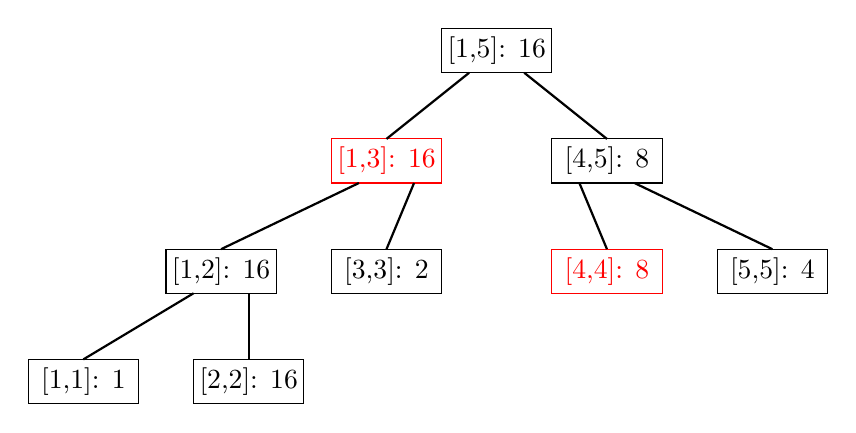
\begin{tikzpicture}[scale=0.7]
          \draw [black] (-1,7.9) rectangle (1,7.1) node [black, midway] {[1,5]: 16}; % Draws a rectangle

          \draw [red] (-3,5.9) rectangle (-1,5.1) node [red,midway] {[1,3]: 16}; % Draws a rectangle
          \draw [black] (1,5.9) rectangle (3,5.1) node [black,midway] {[4,5]: 8}; % Draws a rectangle

          \draw [black] (-6,3.9) rectangle (-4,3.1) node [black,midway] {[1,2]: 16}; % Draws a rectangle
          \draw [black] (-3,3.9) rectangle (-1,3.1) node [black,midway] {[3,3]: 2}; % Draws a rectangle
          \draw [red] (1,3.9) rectangle (3,3.1) node [red,midway] {[4,4]: 8}; % Draws a rectangle
          \draw [black] (4,3.9) rectangle (6,3.1) node [black,midway] {[5,5]: 4}; % Draws a rectangle

          \draw [black] (-8.5,1.9) rectangle (-6.5,1.1) node [black,midway] {[1,1]: 1}; % Draws a rectangle
          \draw [black] (-5.5,1.9) rectangle (-3.5,1.1) node [black,midway] {[2,2]: 16}; % Draws a rectangle

          \draw [thick] (-0.5,7.1) to (-2,5.9);
          \draw [thick] (0.5,7.1) to (2,5.9);

          \draw [thick] (-2.5,5.1) to (-5,3.9);
          \draw [thick] (-1.5,5.1) to (-2,3.9);

          \draw [thick] (1.5,5.1) to (2,3.9);
          \draw [thick] (2.5,5.1) to (5,3.9);

          \draw [thick] (-5.5,3.1) to (-7.5,1.9);
          \draw [thick] (-4.5,3.1) to (-4.5,1.9);
          % \draw [thick] (-2,2) % Draws a line
          % to [out=10,in=190] (2,2)
          % to [out=10,in=90] (6,0) 
          % to [out=-90,in=30] (-2,-2);    
        \end{tikzpicture}
      \end{figure}
    \item 好像可以由蠻少數量的區間得到答案ㄋㄟ,可是具體是多小呢?
  \end{itemize}
\end{frame}

\begin{frame}{\btitle{查詢}}
  \begin{itemize}
    \item 把選法說的具體一點:
      \begin{itemize}
        \item 從根往下看
        \item 每當看到一個被詢問區間完全包含的節點時,就直接使用該節點的答案
        \item 否則就嘗試左右遞迴取出比較好的區間
      \end{itemize}
  \end{itemize}
\end{frame}

\begin{frame}{\btitle{查詢三步驟}}
  \begin{itemize}
    \item 目標:區間詢問 \([ql,qr]\)(\(ql \leq qr\)) 的最大值
    \item 假設目前的節點儲存的資訊是 \([L, R]\)
    \item 查詢三步驟:
    \begin{enumerate}
      \item
        如果 \([L, R]\) 完整的被 \([ql, qr]\) 包含,即 \(ql \leq L \leq R \leq qr\),那麼我們可以直接取用這個節點的最大值。
      \item
        如果 \([L, R]\) 完全跟 \([ql, qr]\) 沒有交集,那麼可以退出遞迴了。
      \item
        否則,遞迴往兩個子樹求解。
    \end{enumerate}
  \end{itemize}
\end{frame}

\begin{frame}{\btitle{查詢三步驟}}
  \begin{itemize}
    \item 複雜度是多少呢?
    \item 很神奇的是,答案可以由 $O(\log N)$ 個預處理資料得到,並且從根走到 + 走完這 $O(\log N)$ 個資料還是 $O(\log N)$
    \item 很神奇的結論!證明記不起來沒關係
    \item \textbf{這就是線段樹的精隨:他可以把一個大區間拆成 $O(\log N)$ 個小區間!}
  \end{itemize}
\end{frame}

\begin{frame}{\btitle{查詢時間複雜度證明}}
  \begin{itemize}
    \item 先找到一個節點 $M$,詢問區間的所有值都在以這個節點為根的子樹裡面,而且這個點要盡量的深(白話文:盡量剛剛好包住詢問區間)
    \begin{itemize}
      \item 從根走到 $M$ 路上只會一直 3.
      \item 用 3. 之後的左右子樹,一個會進到 3.,另外一個進到 2.
      \item 樹深最多 $O(\log N)$,因此最多只會碰到 $O(\log N)$ 個節點
    \end{itemize}
    \item 從 $M$ 開始後,查詢區間其實就被切成左半邊跟右半邊。
    \item 左半邊其實是從 $M$ 的 $mid$ 往左的某段後綴
    \item 右半邊其實是從 $M$ 的 $mid + 1$ 往右的某段前綴
    \item 而後綴 / 前綴的好處是,每當 3. 發生時,左右子樹一定至少有一個是 1. 或 2.
    \item 而 3. 在每個深度最多只會發生一次,所以整題複雜度還是 $O(\log N)$
    \item 整體而言,詢問區間只需要由 $O(\log N)$ 個小區間構成,而造訪這些小區間的複雜度也是 $O(\log N)$!
  \end{itemize}
\end{frame}

\begin{frame}[fragile]{\btitle{範例實作}}
  \begin{minted}[breaklines]{cpp}
    int query(Node *nd, int ql, int qr, int l, int r) {
      if (r < ql || l > qr)   // 完全不包含
        return -inf;
      if (ql <= l && r <= qr) // 完全包含
        return nd->mx;
      int m = (l + r) / 2;
      return max(query(nd->lc, ql, qr, l, m), query(nd->rc, ql, qr, m + 1, r)); // 左右遞迴
    }
  \end{minted}
\end{frame}

\end{document}
